\documentclass[11pt]{article}
\usepackage[margin=2.7cm]{geometry}
\usepackage[T1]{fontenc}
\usepackage[utf8]{inputenc}
\usepackage{lmodern,amsmath,amssymb,amsthm,graphicx}
\usepackage[hidelinks]{hyperref}
\newtheorem{proposition}{Proposition}
\theoremstyle{remark}\newtheorem*{remark}{Remark}
\newcommand{\Z}{\mathbb{Z}}
\title{Directed noise can destroy ergodicity:\\ the absorbing state in Bérard--Dembin--Marêché cannot be dropped}
\author{counterexamples-ips, entry 0003}
\date{Status: \emph{plausible} (not yet checked by a human)\\[2pt]\small Idea: Jonas Köppl. Write-up: Claude (Opus 5.5), 2 November 2026}
\begin{document}
\maketitle

\paragraph{Question.} Bérard, Dembin and Marêché (arXiv:2510.11424) prove: if a finite-range monotone IPS on $\{0,1\}^{\Z^d}$ with $\mathbf 0$ absorbing is ergodic, then adding \emph{directed noise} (each site is set to $0$ at rate $\varepsilon$, i.e.\ $c_0\mapsto c_0+\varepsilon$) gives an exponentially ergodic IPS, for every $\varepsilon>0$. Does this remain true without the absorbing state, i.e.\ for every monotone ergodic $L$? The answer is \emph{no}, already for plain ergodicity.

\paragraph{Setting.} Write $0\leftrightarrow-1$, $1\leftrightarrow+1$ and $S_x(\eta)=\sum_{|y-x|=1}(2\eta(y)-1)$. For $\beta\ge0$, $h\in\mathbb R$ let $L^{\beta,h}$ have rates
\[
c_1(x,\eta)=e^{2\beta S_x(\eta)+2h}\quad(-1\to+1),\qquad c_0(x,\eta)=1\quad(+1\to-1).
\]
The down-rate is constant; this is not heat-bath dynamics. The system is nearest-neighbour, monotone, with positive rates, and $\mathbf 0$ is not absorbing.

\paragraph{Key identity: directed noise is a field.} Adding noise towards $0$ turns $c_0=1$ into $1+\varepsilon$, so
\[
\bigl(L^{\beta,h}\bigr)_\varepsilon=(1+\varepsilon)\,L^{\beta,\,h-\frac12\log(1+\varepsilon)} .
\]

\begin{proposition}
Let $d\ge2$, $\beta>\beta_c(d)$, $\varepsilon>0$, and $L:=L^{\beta,h}$ with $h:=\frac12\log(1+\varepsilon)$, i.e.\ $c_1=(1+\varepsilon)e^{2\beta S_x}$, $c_0\equiv1$. Then
\begin{enumerate}
\item $L$ is monotone, finite range, with positive rates, and ergodic;
\item $L_\varepsilon=(1+\varepsilon)L^{\beta,0}$ is not ergodic: $\mu^+_{\beta,0}\ne\mu^-_{\beta,0}$ are both reversible;
\item $L_{\varepsilon'}$ is ergodic for every $\varepsilon'\ge0$, $\varepsilon'\ne\varepsilon$.
\end{enumerate}
\end{proposition}

\begin{proof}
\emph{Step 1 (reversibility).} In $\pm1$ notation the flip rate satisfies $c(x,\sigma)\,e^{\sigma_x(\beta S_x+h)}=e^{\beta S_x+h}$, independent of $\sigma_x$. So $L^{\beta,h}$ is a stochastic Ising model, and every Gibbs measure for $(\beta,h)$ is reversible, hence stationary (Liggett 1985, Ch.~IV).

\emph{Step 2 (sandwich).} $L^{\beta,h}$ is attractive, so it is ergodic iff $\underline\nu=\overline\nu$ (Liggett 1985, Ch.~III). Compare the process from $\mathbf 1$ with the dynamics in a box $\Lambda$ with spins outside frozen at $+1$. The latter dominates by the comparison theorem, and it converges to the finite-volume Gibbs measure $\mu^+_\Lambda$. Letting $\Lambda\uparrow\Z^d$ gives $\overline\nu\le\mu^+_{\beta,h}$; symmetrically $\underline\nu\ge\mu^-_{\beta,h}$. Hence $\mu^-_{\beta,h}\le\underline\nu\le\overline\nu\le\mu^+_{\beta,h}$.

\emph{Step 3.} For $h\ne0$ the Gibbs measure is unique at every $\beta$ (Lee--Yang; Lebowitz--Martin-Löf), so the sandwich gives ergodicity of $L$ and of $L_{\varepsilon'}=(1+\varepsilon')L^{\beta,h'}$, $h'=\frac12\log\frac{1+\varepsilon}{1+\varepsilon'}\ne0$. For $h=0$ and $\beta>\beta_c$ the plus and minus states differ (Peierls), and both are stationary for $L_\varepsilon$ by Step~1.
\end{proof}

\begin{remark}
Without Lee--Yang: the pressure is convex in $h$, hence differentiable off a countable set, where the Gibbs measure is unique. This gives the counterexample for all but countably many $\varepsilon$.
\end{remark}

\paragraph{Concrete instance.} $d=2$, $\beta=\frac12>\beta_c\approx0.441$, $\varepsilon=1$: flip $+1\to-1$ at rate $1$ and $-1\to+1$ at rate $2e^{S_x}$. This is ergodic; adding rate-$1$ noise towards $-1$ makes it non-ergodic.

\begin{figure}[h]
\centering
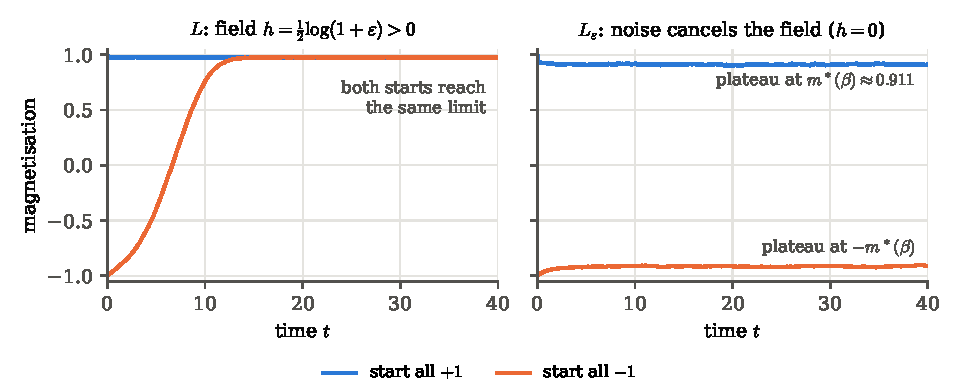
\includegraphics[width=\textwidth]{code/magnetisation.pdf}
\caption{Simulation of the concrete instance on a $200\times200$ torus (\texttt{code/simulate.py}). Under $L$ both starts reach the same limit; under $L_\varepsilon$ they stay at the Onsager--Yang values $\pm m^*(\beta)\approx\pm0.911$. On a finite torus these plateaux are metastable states; the figure illustrates, it does not prove.}
\end{figure}

\paragraph{Mechanism.} Because the down-rate is constant, extra down-flips only rescale it, and a rescaled ratio $c_1/c_0$ is exactly a shift of the field. The noise moves the ergodic system at $h>0$ onto the coexistence line $h=0$. In the absorbing case the noise pushes towards the unique stationary measure $\delta_{\mathbf 0}$ and can only help. Without an absorbing state the non-ergodic set can lie between $L$ and $L_\varepsilon$, and ergodicity is not monotone in~$\varepsilon$. With heat-bath rates the trick fails: $c_1/(c_0+\varepsilon)$ is no longer of Ising form. (Spin-flipped version: constant rate $-1\to+1$, noise towards $+1$.)

\paragraph{What this does not show.} The open question of Bérard--Dembin--Marêché (Sect.~1.5) asks for \emph{some} arbitrarily small perturbation that is exponentially ergodic. Here $L_{\varepsilon'}$ is ergodic for $\varepsilon'<\varepsilon$, so that question remains open.

\paragraph{Follow-up questions.} See \texttt{followups.md} in the entry folder.

\begin{thebibliography}{9}\small
\bibitem{BDM} J.~Bérard, B.~Dembin, L.~Marêché, Sharpness for monotone absorbing interacting particle systems, arXiv:2510.11424 (2025).
\bibitem{H22} I.~Hartarsky, Bootstrap percolation, probabilistic cellular automata and sharpness, \emph{J.\ Stat.\ Phys.}\ 187 (2022).
\bibitem{L85} T.~M.~Liggett, \emph{Interacting Particle Systems}, Springer, 1985, Ch.~III and IV.
\bibitem{LY} T.~D.~Lee, C.~N.~Yang, Statistical theory of equations of state and phase transitions II, \emph{Phys.\ Rev.}\ 87 (1952).
\bibitem{LML} J.~L.~Lebowitz, A.~Martin-Löf, On the uniqueness of the equilibrium state for Ising spin systems, \emph{Comm.\ Math.\ Phys.}\ 25 (1972).
\bibitem{P36} R.~Peierls, On Ising's model of ferromagnetism, \emph{Proc.\ Cambridge Philos.\ Soc.}\ 32 (1936).
\end{thebibliography}
\end{document}
